% !TEX TS-program = pdflatex
% !TEX encoding = UTF-8 Unicode

% This is a simple template for a LaTeX document using the "article" class.
% See "book", "report", "letter" for other types of document.

\documentclass[11pt]{article} % use larger type; default would be 10pt

\usepackage[utf8]{inputenc} % set input encoding (not needed with XeLaTeX)

%%% Examples of Article customizations
% These packages are optional, depending whether you want the features they provide.
% See the LaTeX Companion or other references for full information.

%%% PAGE DIMENSIONS
\usepackage{geometry} % to change the page dimensions
\usepackage{graphicx}
\geometry{a4paper} % or letterpaper (US) or a5paper or....
% \geometry{margin=2in} % for example, change the margins to 2 inches all round
% \geometry{landscape} % set up the page for landscape
%   read geometry.pdf for detailed page layout information

\usepackage{graphicx} % support the \includegraphics command and options

% \usepackage[parfill]{parskip} % Activate to begin paragraphs with an empty line rather than an indent

%%% PACKAGES
\usepackage{booktabs} % for much better looking tables
\usepackage{array} % for better arrays (eg matrices) in maths
\usepackage{paralist} % very flexible & customisable lists (eg. enumerate/itemize, etc.)
\usepackage{verbatim} % adds environment for commenting out blocks of text & for better verbatim
\usepackage{subfig} % make it possible to include more than one captioned figure/table in a single float
% These packages are all incorporated in the memoir class to one degree or another...

%%% HEADERS & FOOTERS
\usepackage{fancyhdr} % This should be set AFTER setting up the page geometry
\pagestyle{fancy} % options: empty , plain , fancy
%\setlength{\headheight}{-25pt}
\renewcommand{\headrulewidth}{0pt} % customise the layout...
\lhead{}\chead{}\rhead{}
\lfoot{}\cfoot{\thepage}\rfoot{}

%%% SECTION TITLE APPEARANCE
\usepackage{sectsty}
\allsectionsfont{\sffamily\mdseries\upshape} % (See the fntguide.pdf for font help)
% (This matches ConTeXt defaults)

%%% ToC (table of contents) APPEARANCE
\usepackage[nottoc,notlof,notlot]{tocbibind} % Put the bibliography in the ToC
\usepackage[titles,subfigure]{tocloft} % Alter the style of the Table of Contents
\renewcommand{\cftsecfont}{\rmfamily\mdseries\upshape}
\renewcommand{\cftsecpagefont}{\rmfamily\mdseries\upshape} % No bold!

%%% END Article customizations

%%% The "real" document content comes below...

\title{Homework 3}
\author{Maksim Levental}
%\date{} % Activate to display a given date or no date (if empty),
         % otherwise the current date is printed 

\usepackage{listings}
\usepackage{color}

\definecolor{dkgreen}{rgb}{0,0.6,0}
\definecolor{gray}{rgb}{0.5,0.5,0.5}
\definecolor{mauve}{rgb}{0.58,0,0.82}

\lstset{frame=tb,
  language=C++,
  aboveskip=3mm,
  belowskip=3mm,
  showstringspaces=false,
  columns=flexible,
  basicstyle={\small\ttfamily},
  numbers=none,
  numberstyle=\tiny\color{gray},
  keywordstyle=\color{blue},
  commentstyle=\color{dkgreen},
  stringstyle=\color{mauve},
  breaklines=false,
  breakatwhitespace=false,
  tabsize=3,
  frame=0
}

\begin{document}
\maketitle

\section*{Problem 1}
If the quantum is not some integer multiple of the timer interrupt period then the process will run for longer than its alotted quantum. For example if the quantum is 101ms and the timer interrupt period is 10ms. Then when on the the 10th time the scheduler wakes to see how much time the process has left, it does not reschedule the process, because it has 1ms left, but also does not wake again for another 10ms. So the process runs for a total of 110ms, an overage of 9ms. So the upper bound on the runtime of the process is ceilingFunction(q/(1/f))*(1/f)=ceilingFunction(q/p)*p where p = 1/f the period of the timer interrupt.

\section*{Problem 2}
For a shorter response time an application with a GUI should be given high priority. Something like a game should get the highest priority because of how critical responsiveness is to the user experience.

For high throughput a web server application should get highest priority so that remote users accessing files on the server can be served quickly and in high volume.

For increased resource utilization priority should be given to applications that are resource intensive applications like MP3 players, video recording software, Internet games.
\section*{Problem 3}

A relocation loader is a loader that adjusts memory addresses in programs in operating systems where partitioned memory management is used. This is done to compensate for variations in addresses at which the loading starts when repeat calls of the program are put into different partitions, with different start addresses. 

Relocation is an alternative boundary registers because boundary registers are used to make sure that programs don't write and read to/from memory addresses that are beyond those belonging to them, that is to say beyond its own memory partition. They are also used to adjust reference addresses by adding the base address to all addresses referenced by the process in order to be inside the memory partition of the process.

\section*{Problem 4}
There are 64K/4K = 16 pages in the virtual address space of process that's running. But there is only room for 32K/4K = 8 page frames in main memory. The virtual address space goes from 0 to 64*1024 - 1 = 65535 with pages having width 4096 and the first page going from 0 to 4095, the second 4096 to 8191, etc. 

\subsection*{a}

31460/4096 = 7.68 so this virtual address is in the 7th page. This page is not in a page frame because there is no entry for the 7th page in the page table. So this instruction would cause a page fault.

\subsection*{b}

17400/4096 = 4.24 so this virtual address is in the 4th page. This page is in the page table as (4,4) so it's in page frame 4. The offset is 17400\% 4096 = 1016 and the physical address is 17400.

\subsection*{c}

45100/4096 = 11.0107 so this virtual address is in the 11th page. This page is in the page table as (11,7) so its page frame is 7. The offset is 45100\% 4096 = 44 and the physical address is (7*4096)+ 44 = 28716

\subsection*{d}

25000/4096 = 6.1035 so this virtual address is in the 6th page. This page is not in a page frame because there is no entry for the 7th page in the page table. So this instruction would cause a page fault.

\section*{Problem 5}

\noindent \scalebox{.59}{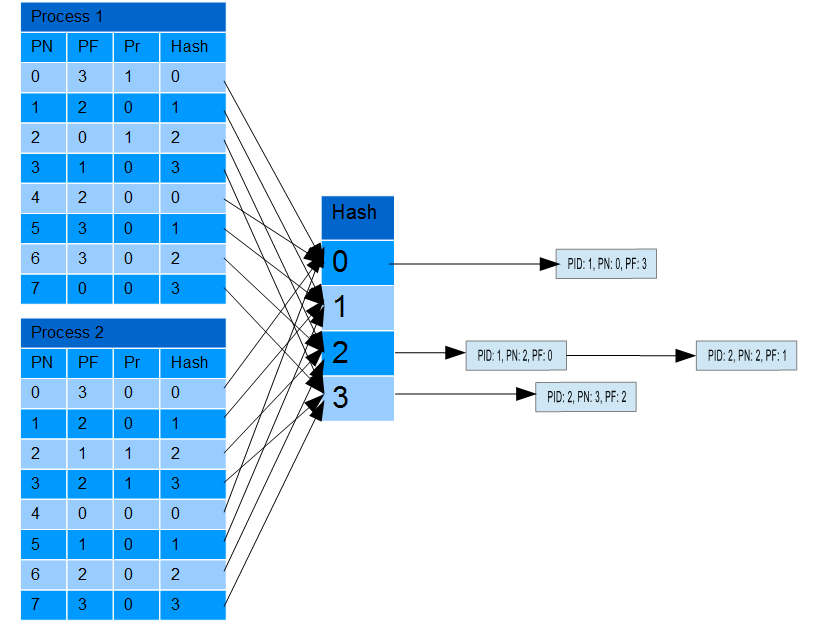
\includegraphics{Untitled.png}}

\end{document}
